\documentclass[a4paper,onecolumn]{article}

\usepackage{amsmath} 
\usepackage{amssymb} 
\usepackage{amsthm}
\usepackage{amsfonts}
\usepackage{graphicx}
\usepackage{subfigure}
\usepackage{subfigmat}
\usepackage{framed}
\usepackage[usenames,dvipsnames]{color}
\usepackage[textsize=small]{todonotes}
\usepackage{algorithm, algorithmic}
\numberwithin{algorithm}{section}
\usepackage{enumerate}
\usepackage{url}
%\usepackage{xcolor}
\usepackage[margin=3.5cm]{geometry}

\theoremstyle{plain}
\newtheorem{lem}{Lemma}
\newtheorem{thm}{Theorem}
\newtheorem{prop}{Proposition}
\theoremstyle{definition}
\newtheorem{defi}{Definition}
\newtheorem{problem}{Problem}
\newtheorem{assume}{Assumption}
\newtheorem{corollary}{Corollary}
\newtheorem{claim}{Claim}
\newtheorem{fact}{Fact}
\newtheorem{remark}{Remark}
\theoremstyle{example}
\newtheorem{example}{Example}
\newtheorem{obs}{Observation}


\newcommand{\Z}{\makebox[0.06cm][l]{\sf Z}{\sf Z}}
\newcommand{\Prob}{\makebox[0.06cm][l]{\sf P}{\sf P}}
\newcommand{\CS}{\mathcal{S}}
\newcommand{\CZ}{\mathcal{Z}}
\newcommand{\R}{\mathbb{R}}
\newcommand{\N}{\mathbb{N}}
\newcommand{\B}{\mathcal{B}}
\newcommand{\gam}{\gamma}
\newcommand{\bb}{\beta}
\newcommand{\oo}{\omega}
\newcommand{\lam}{\lambda}
\newcommand{\al}{\alpha}
\newcommand{\eps}{\epsilon}
\newcommand{\del}{\delta}
\newcommand{\sig}{\sigma}
\newcommand{\sgn}{\text{sgn}}
\newcommand{\m}{\mathcal}
\newcommand{\mb}{\mathbf}
\newcommand{\demand}{x}
\newcommand{\Demand}{\mathcal{X}}
\newcommand{\price}{p}
\newcommand{\cost}{J}
\newcommand{\nmech}{M}
\newcommand{\dpmech}{\nmech_{\eps,\delta}}
\newcommand{\neigh}{\mathcal{N}}
\newcommand{\sense}{\Delta}
\newcommand{\lmech}{\nmech^{L}_\eps}
\newcommand{\emech}{\nmech^{E}_\eps}
\newcommand{\pmech}{\nmech^{P}_\eps}
\newcommand{\baseline}{b}
\newcommand{\abs}[1] {\left|#1\right|}
\newcommand{\cset}[2] {\left\{#1 ~\middle|~ #2\right\}}
\newcommand{\maryam}[1]{\todo[inline,color=blue!20]{MK:\ #1}}
\newcommand{\christos}[1]{\todo[inline,color=red!20]{CD:\ #1}}
\newcommand{\maryamm}[1]{\todo[color=blue!20]{MK:\ #1}}
\newcommand{\christosm}[1]{\todo[color=red!20]{CD:\ #1}}

\newcommand{\Laplace}{\textrm{Laplace}}


\begin{document} 
\title{Notes: Pricey of Privacy in Real-time Electricity Markets}

\author{Christos and Maryam}
\maketitle

\section{Introduction.}

We consider the problem of privacy for households participating in
smart grid system. From the point of view of the households, there are
two distinct problems: firstly, how much privacy do they lose in
general by participating in an online price mechanism? Secondly, given
that they participate in the mechanism, how much privacy can they
expect with respect to their household occupancy?

We consider price models that depend on the total consumption of electricity. Such models have been studied in so and so. 

There are two types of privacy that we might like to model. The first
is pure data privacy: we wish to give an incentive to participants to
submit their data to a mechanism, by making sure that the output of the mechanism is only weakly dependent on their data. This is achieved by differential privacy. The second type of privacy is more specific. Given a parametric family of distributions, we wish to protect a specific secret about individuals or groups, such as house occupancy at different times. This goal can be achieved by Pufferfish privacy.

\subsection{Related work}

\paragraph{Privacy.}An algorithm for achieving Pufferfish privacy was presented by~\cite{wang2016privacy}.

\paragraph{Games in electricity markets.} \cite{paccagnan2016aggregative} present an aggregative game where individuals have semi-quadratic cost functions.
\christos{I guess we are dropping the quadratic term?}


\subsection{Differential privacy.}

Let $(P, \Omega, \Sigma)$ be a probability space and $\CS$ a
topological space.  A randomised mechanism
$\nmech : \Omega \times \CS \to \CZ$, is
$(\epsilon, \delta)$-differentially private if, for any two
neighbouring points $x, y \in \CS$
\begin{equation}
  \label{eq:differential-privacy}
  P(\nmech = z \mid x) \leq P(\nmech = z \mid y) e^\epsilon + \delta, \qquad \forall z \in \CZ.
\end{equation}
The notion of neighbourhood is crucial here, as it quantifies what we mean by privacy. Essentially, an $(\epsilon,\delta)$-DP mechanism guarantees that with probability at least $1-\delta$, two neighbouring datasets $x, y$ are $\epsilon$-indistinguishable from each other given the output of the randomised 
mechanism. 


As an example, consider the setting of users $i$ having demand
$\demand_{i,t}$ over different times of the day. They send those
demands to a mechanism, which then sets prices for electricity. Then
we could define their neighbouring datasets as those for which a
single demand $\demand_{i,t}$ is changed. However, this is a very weak
notion of privacy, because it might be easy for an adversary to
distinguish between different demands over multiple
periods. Alternatively, we could define neighbouring datasets as those
for which the demand values $\cset{\demand_{i,t}}{t \in [T]}$ for a
single user $i$ are changed, or missing. This is a more robust
definition, as it essentially tells every participant that the
mechanism is insensitive to their participation. Hence, it will be
hard for an adversary to learn \emph{anything} about their data.



\subsubsection{The Laplace mechanism $\lmech$}

The Laplace mechanism can be used to obtain private versions of any
non-private mechanism $\nmech : \CS \to \R$.
Let $\sense \nmech$ be the sensitivity of the original mechanism 
\[
\sense \nmech = \max_{x N y} |\nmech(x) - \nmech(y)|.
\]
Then the new mechanism is simply:
\[
\lmech(x) = \nmech(x) + \omega, \qquad \omega \sim \Laplace(\sense \nmech / \eps).
\]
The sensitivity depends on how we define neighbourhoods.

\paragraph{Neighbourhood as presence of data} For the definition of
neighbourhood as one field missing or added, and assuming
w.l.o.g. that $\demand_{i,t} \in [0, 1]$, we note that the sensitivity
of the average demand is bounded by $1$, hence the sensitivity is
\begin{align}
  \sense \nmech 
&= \sup_{\demand \neigh \demand'} \abs{M\left(c_t + \frac{1}{N} \sum_{i=1}^N \demand_{i,t}\right) - M\left(c_t + \frac{1}{N-1} \sum_{i=1}^{N-1} \demand_{i,t}\right)}.
\end{align}
Instead of analysing this directly, we can first check the arguments. Their difference for neighbouring datasets is
\begin{align}
 \abs{\frac{1}{N} \sum_{i=1}^N \demand_{i,t} - \frac{1}{N-1} \sum_{i=1}^{N-1} \demand_{i,t}}
  &=
    \abs{\left(\frac{1}{N} - \frac{1}{N-1}\right) \sum_{i=1}^{N-1} \demand_{i,t} + \frac{1}{N} \demand_{N, t}}
  \leq 1.
\end{align}
Then the sensitivity of the overall function is $\sense \nmech = \sup_z \nabla \nmech(z) \times 1$. 

\paragraph{Neighbourhood as value of data}
Note that the corresponding difference for the alternative definition
of neighbourhood (one person changing their data) for a \emph{fixed} population size (i.e. if the number $N$ and identity of people used in the computation is common knowledge) is bounded by $\frac{1}{N}$, and so the overall sensitivity then is  $\sense \nmech = \sup_z \nabla \nmech(z) \times 1/N$. 
This probably makes more sense in our setting. For a linear $M$, Figure~\ref{fig:local-neighbourhood} shows the additional average cost incurred as we change $\epsilon$, \footnote{Note that the price never becomes negative in this particular scheme.} for a fixed demand profile. \christos{Do individuals optimise at each round? I am a bit confused about that.}
\begin{figure}[h]
  \centering
  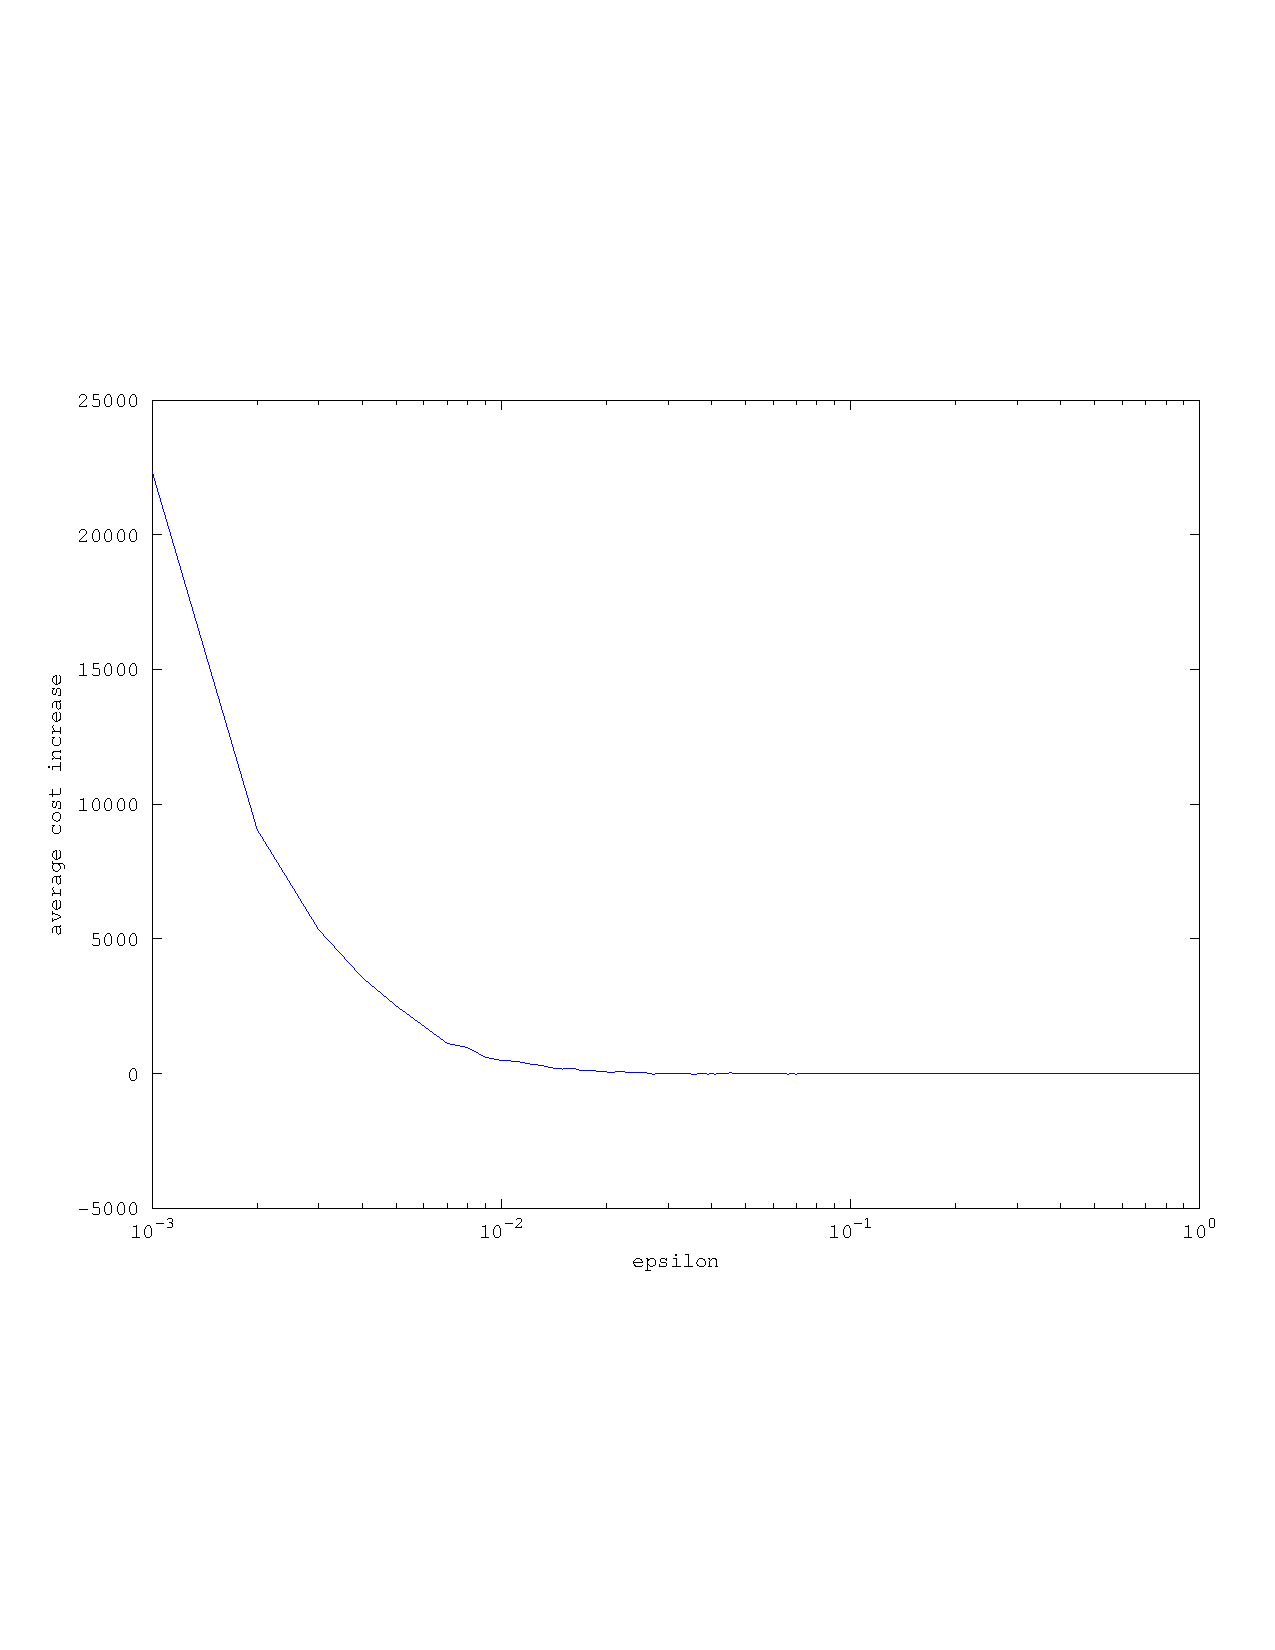
\includegraphics[width=0.6\textwidth]{src/average_cost_increase_linear}
  \caption{Average cost increase}
  \label{fig:local-neighbourhood}
\end{figure}


\subsubsection{The Exponential mechanism $\emech$}
The mechanism is very simple. For a utility function $U(b, p)$, where $b$ is our input (i.e. bids) and $p$ is our decision (i.e. price), then the mechanism selects price $p$ with probability
\begin{equation}
  \label{eq:exponential mechanism}
  \emech(p \mid b) = \frac{e^{\epsilon U(b, p)} \mu(p)}{\int e^{\epsilon U(b, p)} \mu(p) dp},
\end{equation}
where $\mu$ is a base measure.

\paragraph{Handling constraints.}
Using the exponential mechanism, constraints are not particularly
difficult in theory.  The first case is when we have the problem
$\max U(b, p)$ such that $p \in C$. Then we can simply select $\mu$
such that $\mu(p) = 0$ if $p \notin C$.  The second case is
$\max U(b, p)$ such that $f(b, p) \in C$. Then we can use rejection
sampling. However, the problem is that our constraints also depend
upon the private input $b$ of the users. Hence, we must deal with a
randomised version of the constraints. 


\section{Consumption privacy.}

Consider a mechanism that, given the demanded consumption
$\demand_t^i$ of households $i$ at times $t$, decides upon a price
level $\price_{t}$ for that time period, which depends on
$\demand_{t}$. As the mechanism's price level is public knowledge, it
can leak private information about demand (or consumption). For that
reason, we shall consider price-setting algorithms that have privacy
guarantees.

If the mechanism for determining the price level is
$\epsilon$-differentially private for period $t$, the we must have
\[
\left|
  \ln \frac{\Pr(\price_t \mid \demand_t)}{\Pr(\price_t \mid x'_t)}
\right|
 \leq \epsilon
\]
where $\demand_t = (\demand^1_t, \ldots, \demand^n_t)$ is a vector of
bids and/or consumptions of individual households for the $t$-th time
period and $x'_t$ is a vector where the data of one individual is
added or missing.  However this only protects us against one time
period: for $T$ periods, this only guarantees $T \epsilon$
differential privacy.



\subsection{Local differential privacy.}
Local differential privacy ensures that all the data consumers send are already privatised. This is done by randomising the data that they would have sent in the first place. So, instead of user $i$ sending $x_{i,t}$ for their planned consumption at time $i$, they send $y_{i,t} \sim P_{\epsilon, \delta}(x_{i,t})$ from some appropriate distribution.

If the data is planned energy use during different periods, then local privacy is simple to achieve. First we need to define the notion of neighbourhood that we wish to use. This specifies which data we want to protect in the first place.

Let's assume that each user wants to make their daily participation
private, that is that they wish to hide the value of their data for
the whole day. If there are $T$ periods per day, and the range of the
consumption is $C$, we need to add independent Laplace noise with
parameter $TC / \epsilon$ to each consumption period to achieve local
$\epsilon$-differential privacy for the day's data for each user. So,
any participant would be certain that it would be very difficult for
an adversary to learn any more information about his planned
consumption from the published data than he already knew.\footnote{It
  is important to note here that if a person always has the same
  consumption plan every day, then this plan will eventually be
  learned by an adversary. However, applying this specific notion of
  differential privacy ensure that an adversary cannot guess their
  plans any given day from the data they release. If we wish to hide
  average planned consumption, then we must bias the data we send
  every day in a fixed way.}

If the price at each time period is only a function of average demand,
then it's easy to see that the estimation error due to privacy is
going to be $O(TC / \epsilon \sqrt{n})$.


\subsection{The price setting mechanism.}
The price-setting mechanism needs to be differentially private. The simplest way is to use the exponential mechanism. The utility of the price-setter is to ensure the demand peak is low.. this can be achieved by having a utility function $\left(\baseline_t + \frac{1}{N}\sum_{i=1}^N \demand_{i,t}\right)^2$, where $\baseline_t$ is an inflexible power demand and $\demand_{i,t}$ is the power demand of customer $i$ at time $t$. 
In general, a price-setting mechanism $\nmech$ itself determines the price $\price_t$ at time $t$ in a manner dependent upon a baseline price $\baseline_t$ at time $t$ and $\demand_{i,t}$, the expected demand by use $i$ at time $t$.
\[
\price_t = \nmech\left(\baseline_t + \frac{1}{N}\sum_{i=1}^N \demand_{i,t}\right),
\]


The baseline price may in turn depend on the overall supply and demand
for the time of day, while the individual demands are estimated from
local consumer data.  The cost for the $i$-th consumer is going to be
\[
\cost_i(\demand_i) = \sum_{t=1}^T \price_t \demand_{i,t}
\]
If we wish the price to be differentially private with respect to an individual's demand (at any given time period) then there are two standard methods whereby we can achieve this. The first is through adding Laplace noise to the price determined by the non-private mechanism $\nmech$. The second is by formulating the problem as an optimisation problem, whose solution as $\eps \to \infty$ converges to the mechanism $\nmech$.

\maryam{can someone by observing price only (which depends on the average of demand) learn something about individual demands $\demand_{i,t}$?}
\christos{Yes. The trivial case if if they know all other demands.}

\paragraph{Auctions between electricity providers and the transmission
  system.} We have $N$ participants with bids $B_j = (x_j, c_j)$,
where $p_j$ is the vector of offered \christosm{I suppose also
  requested?} supplies and $c_j$ that of requested costs.  Given the
set of all bids $B$, the choice function $F(B) \in 2^B$ tells us which
bids we accept.\christosm{What does it mean to accept two different
  bids by a participant?}  The utility of each participant is
\[
u_j(B) = q_j(B) - \bar{c}_j%\top f_j(B)
\]
where $q$ is a payment function and $\bar{c}$ is the true cost (which the participant may want to hide?). The transmission system's cost is
\[
U(x, y, B) = c^\top + D(x, y),
\]
where $x \in \{0, 1\}^n$ selects the accepted bids\christos{Same as $f(B)$?}, $y$ is additional variables, and $D$ is an arbitrary real function \christos{But we should probably restrict it to smooth functions.}

\paragraph{Auctions between consumers and providers.} Each bidder has a demand curve $b_i: [0,1] \to \R$, with $b_i(p)$ telling us how much power bidder $i$ would like at price $p$. Assuming $b_i$ is non-increasing, and  bounded by $b_i(p) \leq 1/p$, our utility function is
\[
U(b, p) = p \sum_{i=1}^N b_i(p).
\]
Now we can use the exponential mechanism to take care of this.


\subsubsection{The posterior sampling mechanism $\pmech$}
For the case where we wish to base our decision on some statistics, we
can use Bayesian inference to estimate a posterior distribution on the
parameters of interest. Given some regularity conditions on the
parameter space, we can base our decision making on samples from the
posterior in order to guarantee differential privacy.



\section{Occupancy privacy.}
Let the data that smart meters obtain from each household be the energy consumption in kilowatt-hour (KWhr) every $\Delta$ units of time, for example $\Delta = 15$ minutes. Denote this data by $\demand^i_t \in [0, \bar{\demand}]$, where $i$ represents the household and $t$ is the time index. Let occupancy of household $i$ at time $t$ be denoted by $z^i_t \in \{0,1\}$. Let the utility function be denoted by $U^i(\demand^i,y^i) = - | \sum_{t=1}^T (\demand^i_t-y^i_t)\price_t|$, where $\price_t$ denotes the price of electricity at time $t$. This ensures that the customer bill remains close to its true value. Our problem is to maximise the utility, while ensuring occupancy remains private. We formalise this problem as follows. Design $M_t:\R_+ \rightarrow \R_+$ and communicate $y^i_t = M_t(\demand^i_t)$ through the smart meters to utility, with the objectives of minimising probability of finding $\{z^i_t\}_{\tau_1}^{\tau_2}$ from $\{y^i_t\}_{t_1}^{t_2}$ while maximising utility. \maryam{reasonable choice of $t_1, t_2, \tau_1, \tau_2$?}
As all the discussion below corresponds to data from an individual household, from now on, we will drop the index $i$.

Let occupancy evolve according to a two-state Markov chain, with time-dependent transition probability matrix $P^z_t(z_{t+1} | z_t)$. Let electricity consumption evolve according to a Markov process $P_t(\demand_{t+1} |\demand_t, z_t)$. For example, $\demand_t$ can have a truncated normal distribution with mean determined by occupancy and time of day. \maryam{what choices of distribution are accurate representations and  enable efficient computation?}.  \christos{I actually have no idea, but we have to assume some family. It can also be a non-parametric family, e.g. histograms.}

Motivated by the Pufferfish privacy framework \cite{pufferfish_quilt}, let the secret $S$ denote occupancy of a household at a given time $\tau \in [\tau_1, \tau_2]$. Let the secret to hide be represented by $\mathcal{Q} = \{z_{\tau,0}, z_{\tau,1}\}$ , where $0$, $1$  indices indicate no occupancy, occupancy at time $\tau$, respectively. Let $Z = (Z_{\tau_1}, Z_{\tau_1+1}, \dots, Z_{\tau_2})$. Let $\Theta$ denote all probability distributions consistent with the Markov transition kernel $P_t$ defined above. Let $\demand = (\demand_{t_1}, \demand_{t_1+1}, \dots, \demand_{t_2})$,  $y = (y_{t_1}, y_{t_1+1}, \dots, y_{t_2})$. we call a mechanism $M: \Demand \rightarrow Y$ $\epsilon$-Pufferfish private if $\forall W \subset \text{Range}(M)$, and datasets $\demand \sim \theta$, with $\theta \in \Theta$
\begin{align*}
e^{-\epsilon} \leq \frac{P(M(\demand) \in W|Z_\tau=0, \theta )}{P(M(\demand) \in W|Z_\tau=1, \theta)} \leq e^{\epsilon}.
\end{align*}
We need the above to hold for any $\tau \in [\tau_1, \tau_2]$, meaning  that we wish to hide the occupancy of a household for a given time period.

In the Pufferfish paper, this class of problems are addressed by adding Laplacian noise to data, where the scale of the noise is dependent on the maximum Wasserstein distance $W$, between two densities in $\Theta$.  \maryam{Does this approach map to our setting? If so, how do we compute $W$? Are there other ways to ensure Pufferfish privacy? What is the loss in utility? }

\bibliographystyle{plain}
\bibliography{references}



\end{document}

%%% Local Variables:
%%% mode: latex
%%% TeX-master: t
%%% End:
